
In recent years, VMC methods leveraging NQS have been developed to model the wave functions of complex nuclear systems with high accuracy and favorable polynomial scaling with the number of nucleons. Similar to conventional continuum QMC methods, working in coordinate space enables NQS-based approaches to efficiently capture short-range nuclear dynamics. As illustrated schematically in Fig.~\ref{fig:nqs_schematic}, NQS architectures typically take as input the spatial and spin-isospin coordinates of the nucleons and output the amplitude and phase of the quantum many-body wave function. A generic neural-network architecture with this construction will not guarantee fermion anti-symmetry, so it must be explicitly imposed. To this aim, in parallel with condensed-matter and quantum-chemistry applications, different ans\"atze, discussed in detail in Section~\ref{sec:wavefunction}, have been developed. 

In contrast, in second-quantized approaches, fermion antisymmetry is encoded directly by the basis and the operator algebra: states are expanded in the ordered occupation basis, and fermionic signs follow from the canonical anticommutation relations upon reordering operators. Consequently, in second quantization no additional permutation constraint is imposed on the variational wave function. The fermionic signs are determined by the ordered Fock basis and the anticommutation relations, not by any symmetry of the coefficients~\cite{choo_fermionic_2020}. 

\begin{figure}[!hb]
    \centering
    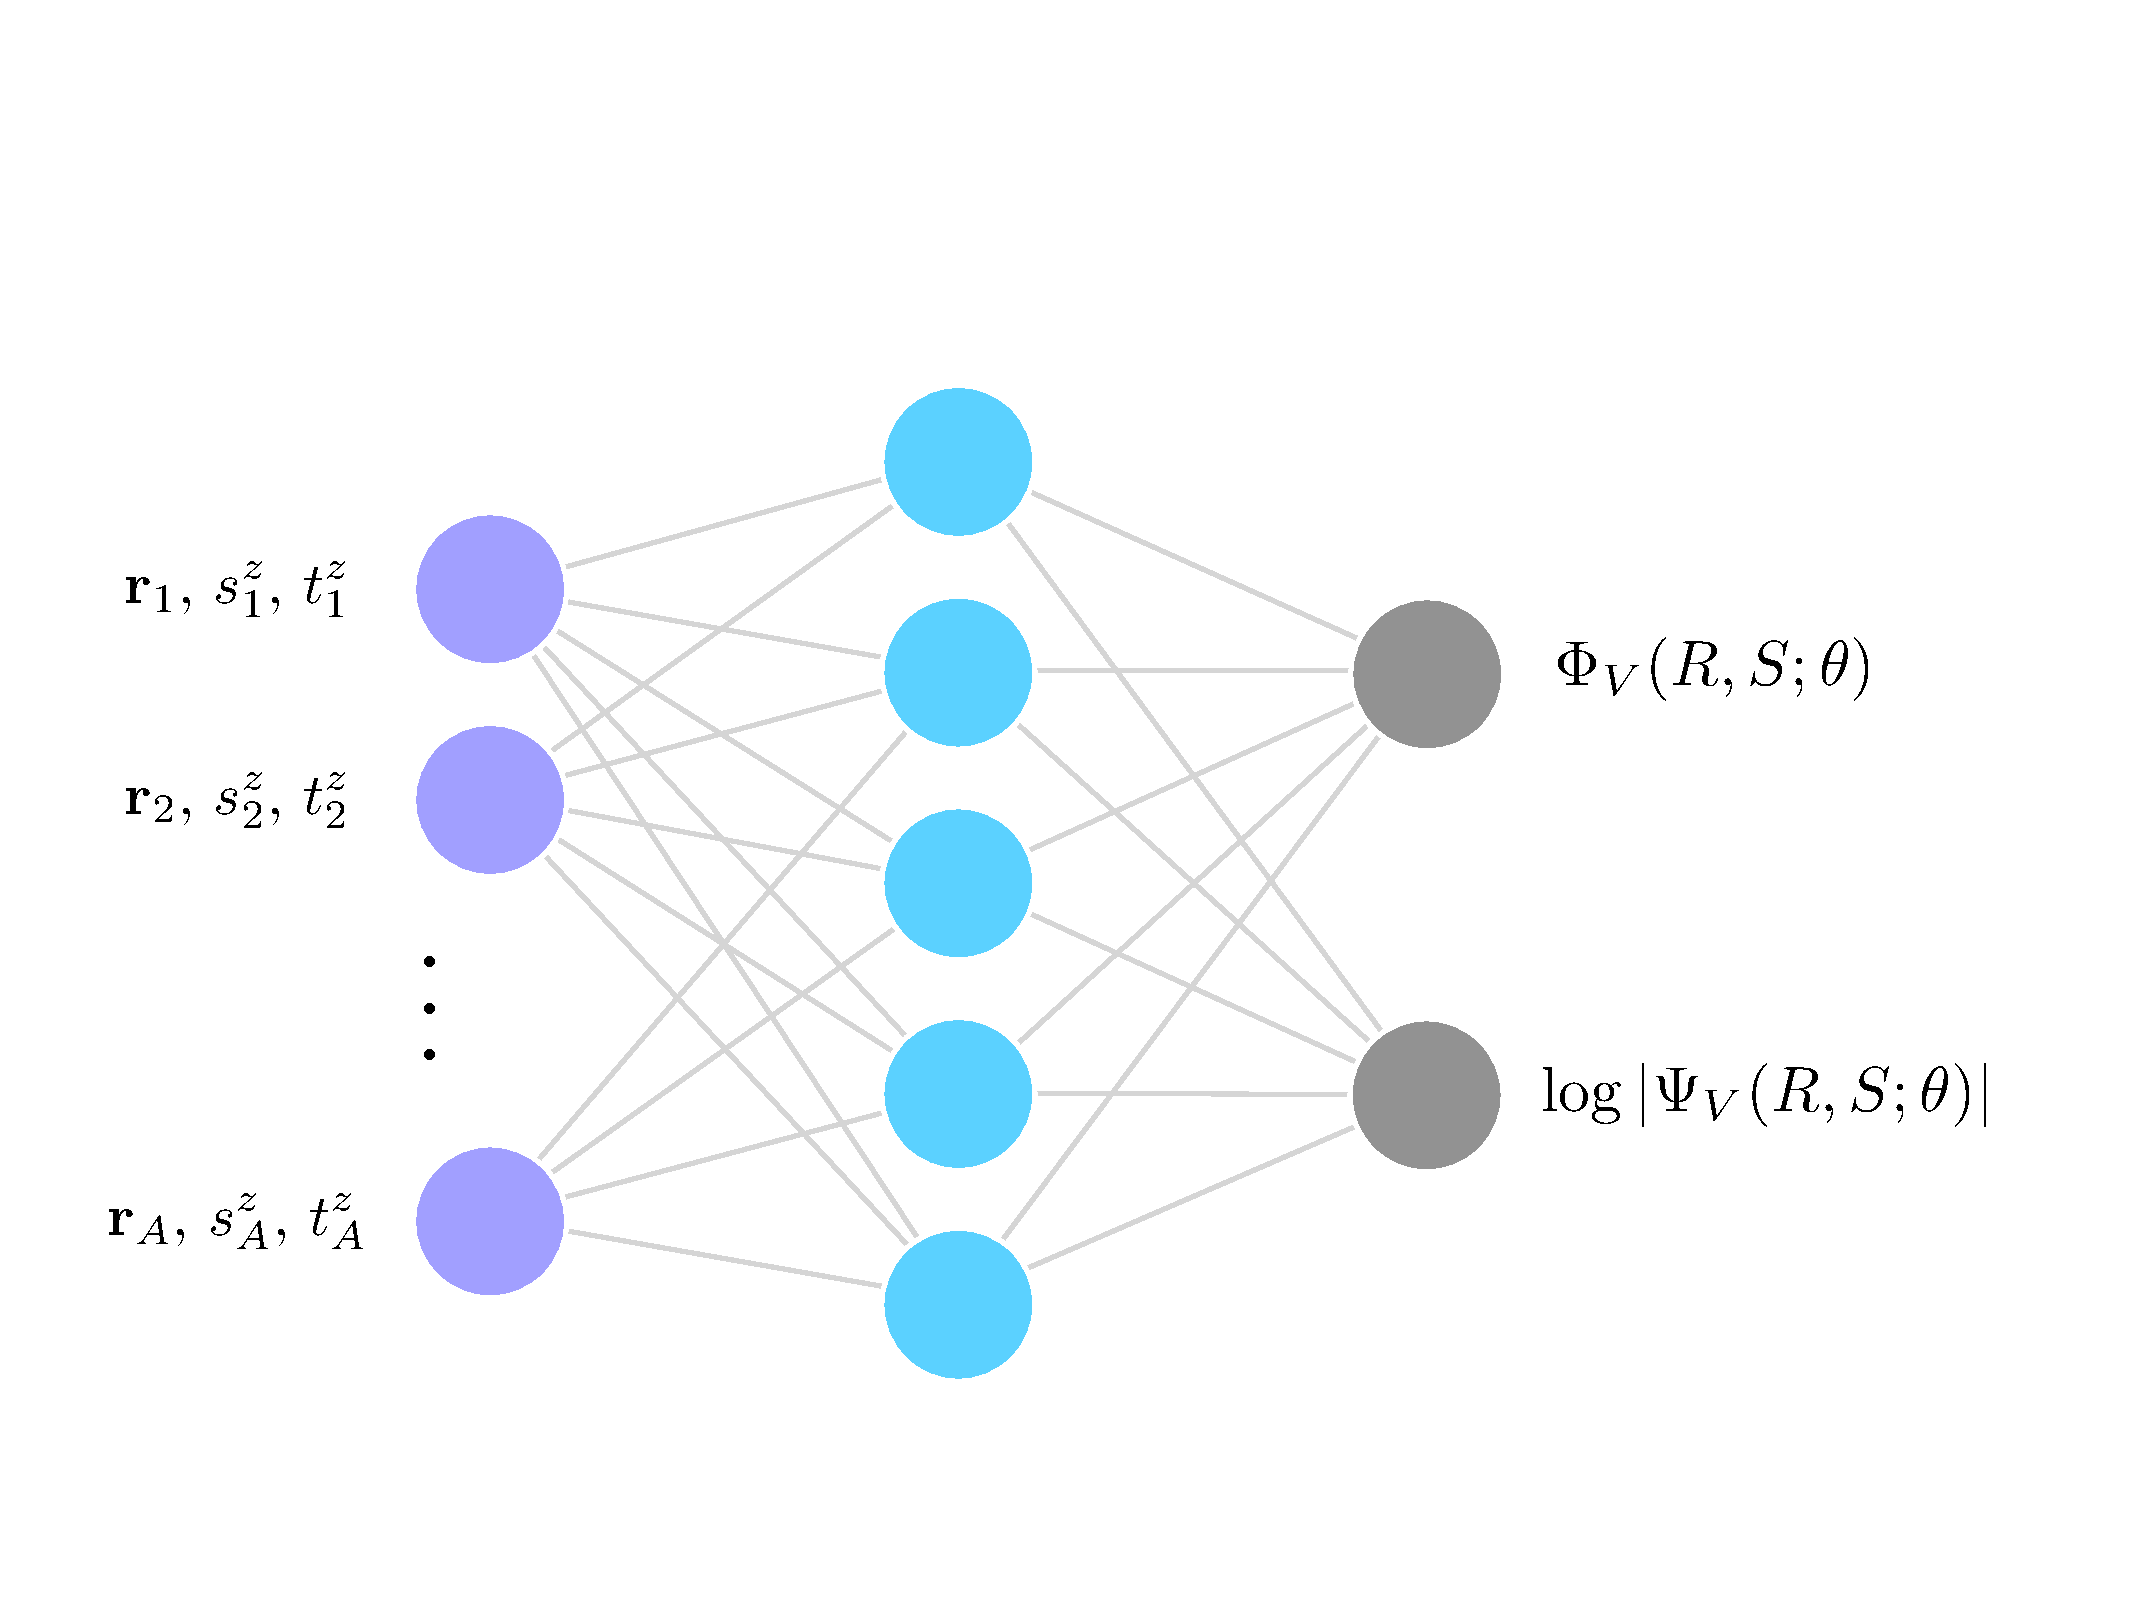
\includegraphics[width=0.7\linewidth]{figures/neural_quantum_states/network_cropped.pdf}
\caption{Schematic representation of a NQS to solve the nuclear quantum many-body problem. An anti-symmetric artificial neural network takes as input the spatial and spin-isospin coordinates of the  $A$ nucleons, $\{\mathbf{r}_i, s^z_i, t^z_i\}$, and outputs the logarithmic amplitude and phase of the quantum many-body wave function, $\log(\Psi_V(R\, S;\theta)) = \log|\Psi_V(R\, S;\theta)| + i\Phi_V(R\, S;\theta)$
\label{fig:nqs_schematic}}


\end{figure}
  
\subsection{Sampling the Hilbert space }
Evaluating the variational energy in Eq.~\eqref{eq:variational} requires
carrying out a $3A$-dimensional integral over the continuous Cartesian
coordinates of the nucleons,
$R = (\mathbf{r}_1, \ldots, \mathbf{r}_A)$,
and a sum over the $2^A \binom{A}{Z}$ discrete spin--isospin configurations,
$S=\big((s_1^z, t_1^z), \ldots, (s_A^z, t_A^z)\big),$
with $s_i^z$ and $t_i^z$ denoting the spin and isospin projections of the $i$th nucleon:
\begin{equation}
E_V =
\frac{\langle \Psi_V | H | \Psi_V \rangle}{\langle \Psi_V | \Psi_V\rangle}
= \frac{\sum_{S} \int dR\, \langle \Psi_V | R S\rangle \langle R S | H | \Psi_V\rangle}
{\sum_{S} \int dR\, \langle \Psi_V | R S\rangle \langle R S | \Psi_V\rangle},
\label{eq:variational_2}
\end{equation}
where, for brevity, we have dropped the explicit dependence of the variational state on a set of parameters $\params$. Since a deterministic evaluation is computationally prohibitive, these expressions are estimated stochastically using Monte Carlo sampling. To this end, it is convenient to rewrite the variational energy as
\begin{equation}
E_V
= \frac{\sum_{S} \int dR\, |\Psi_V(R,S)|^2 \dfrac{\langle R S | H | \Psi_V \rangle}
{\langle R S | \Psi_V \rangle}}
{\sum_{S} \int dR\, |\Psi_V(R,S)|^2}
= \sum_{S} \int dR\, \pi_V(R,S)\, E_L(R,S)\,,
\label{eq:en_exp}
\end{equation}
where we introduced the probability distribution and the local energy,
\begin{equation}
\pi_V(R,S) =
\frac{|\Psi_V(R,S)|^2}{\sum_{S} \int dR\, |\Psi_V(R,S)|^2}\,,
\qquad
E_L(R,S) =
\frac{\langle R S | H | \Psi_V \rangle}{\langle R S | \Psi_V \rangle}\,.
\end{equation}
This procedure is unbiased, since configurations with
$\Psi_V(R,S)=0$ do not contribute to Eq.~\eqref{eq:variational_2}, and the
reweighting by $|\Psi_V(R,S)|^2$ is therefore well defined.

In most NQS-based applications of the VMC method to the nuclear many-body
problem~\cite{adams_variational_2021,Gnech2021,yang_consistent_2022,Yang:2023rlw,
gnech_distilling_2024}, with the notable exception of
Ref.~\cite{wen_neural-network_2025}, the Metropolis--Hastings
algorithm~\cite{metropolis_equation_1953,hastings_monte_1970} is used to
generate Markov chain samples of spatial and spin--isospin configurations
distributed according to $\pi_V(R,S)$. The resulting $N_{\rm conf}$
configurations are then used to estimate ground-state expectation values via
\begin{equation}
E_V \simeq \frac{1}{N_{\rm conf}} \sum_{\{R,S\}\sim \pi_V} E_L(R,S)\, .
\end{equation}


The initial $3A$ spatial coordinates of the nucleons are typically sampled from a Gaussian distribution centered at the origin, with per–coordinate variance chosen to reproduce the target rms point radius. For example, taking $R_{\rm pt}\approx 1.2\,A^{1/3}\,\mathrm{fm}$, one may set $\sigma^2 = R_{\rm pt}^2/3$. The $z$-projections of the spin–isospin degrees of freedom are randomly initialized so that the total charge and total spin of the nucleus of interest are reproduced. Each Monte Carlo step consists of a Gaussian move of the $3A$ spatial coordinates. Since charge is conserved, an ergodic isospin move within fixed $Z$ is to swap the isospin labels of a randomly selected pair of nucleons. The same swap is a legitimate move for the spin labels if tensor and spin–orbit contributions in the NN potential are neglected, so that the total spin projection $S_z=\sum_i s_i^z$ is conserved. However, when tensor or spin–orbit interactions are present, one also needs moves that do not conserve $S_z$, such as single or double spin flips, to ensure ergodicity.

The newly proposed spatial configuration $R'$ and spin–isospin projection $S'$ are accepted separately (in two successive Metropolis updates) with probabilities
\begin{equation}
A(R\!\to\! R')=\min\!\left[1,\frac{|\Psi_V(R',S)|^2}{|\Psi_V(R,S)|^2}\right],\qquad
A(S\!\to\! S')=\min\!\left[1,\frac{|\Psi_V(R,S')|^2}{|\Psi_V(R,S)|^2}\right],
\end{equation}
where we have assumed symmetric proposal kernels for the Gaussian spatial moves. The width of the Gaussian ``kick'' is tuned to keep the spatial acceptance rate near $0.6$.

After $N_{\rm therm}$ thermalization steps, which are necessary to equilibrate the Markov chain, the Metropolis–Hastings algorithm produces configurations $\{R,S\}$ distributed according to the target probability $\pi_V(R,S)$. Because successive samples are correlated, $N_{\rm void}$ ``void'' (non-measurement) steps are typically inserted between measurements, and chosen such that the residual autocorrelation falls below a prescribed threshold. After equilibration, a total of $N_{\rm meas}$ measurements are performed. To improve efficiency, the embarrassingly parallel nature of the Metropolis–Hastings algorithm is exploited by propagating $N_{\rm chains}$ independent Markov chains in parallel, so that the total number of configurations used to estimate observables is
$N_{\rm conf}=N_{\rm chains}\times N_{\rm meas}$.


\subsection{Optimization strategies}
\label{subsec:opt}
The energy estimate in Eq.~\eqref{eq:variational} provides an upper bound to the ground-state energy. One must still minimize this quantity with respect to the parameters $\params$, which turns VMC into a nonlinear optimization problem:
\begin{equation}
E^{*}=\min_{\params}\, E_V(\params)\,, \qquad
\params^{*}=\arg\min_{\params}\, E_V(\params)\, .
\end{equation}
A standard strategy is to solve this problem iteratively. A succinct account of such iterative approaches in the NQS setting is given below. For comprehensive treatments in machine learning and optimization (including non-iterative methods), see Refs.~\cite{nocedal_numerical_2006,amari_information_2016}. 


In an iterative scheme, one starts from an initial parameter vector $\params$ and updates it as
$\params \leftarrow \params + \boldsymbol{\delta}$, where the increment $\boldsymbol{\delta}$ is chosen to reduce the energy objective. In the NQS setting, a common choice is
\begin{equation}
\boldsymbol{\delta} \;=\; -\,\eta\, S^{-1}\, \mathbf{g} \,,
\label{eq:update_pars}
\end{equation}
which corresponds to minimizing the local quadratic model
\begin{equation}
M(\boldsymbol{\delta}) \;=\; E_V(\params) \;+\; \boldsymbol{\delta}^{\top} \mathbf{g} \;+\; \tfrac{1}{2}\, \boldsymbol{\delta}^{\top} S\, \boldsymbol{\delta}\,.
\label{eq:quadratic_sr}
\end{equation}
The scalar $\eta$ is the learning rate that controls the overall step size in parameter space. The gradient of the variational energy is
\begin{equation}
g_i
= 2 \left(
\frac{\braket{\Psi_V | O_i^\dagger H | \Psi_V}}{\braket{\Psi_V | \Psi_V}}
- \frac{\braket{\Psi_V | O_i^\dagger | \Psi_V}}{\braket{\Psi_V | \Psi_V}}
  \frac{\braket{\Psi_V | H | \Psi_V}}{\braket{\Psi_V | \Psi_V}}
\right)\!,
\label{eq:gradient}
\end{equation}
where $O_i|\Psi_V(\params)\rangle = \partial_{\theta_i} |\Psi_V(\params)\rangle$ denotes a derivative of the wave function with respect to $i-$th parameter. The matrix $S$ serves as a preconditioner, and different optimization schemes prescribe different choices. In the information-geometry paradigm, $S$ accounts for the curvature and geometry of parameter space, beyond the Euclidean (flat-space) gradient descent corresponding to $S=I$~\cite{amari_information_2016}. In quadratic optimization, there is also a close relationship between $S$ and the Hessian of the loss function~\cite{nocedal_numerical_2006}.


An extension of the information geometry approach in many-body quantum mechanics is the \emph{stochastic reconfiguration} (SR) method~\cite{stokes_quantum_2020}. Originally and independently introduced in the QMC literature at the end of the last century~\cite{sorella1998,sorella_wave_2005}, SR translates naturally to the NQS setting. It is commonly justified by minimizing the Fubini–Study distance between an updated NQS state and a small imaginary-time step for energy minimization~\cite{sorella1998,stokes_quantum_2020,park_geometry_2020}. This leads to identifying $S$ with the real part of the quantum geometric tensor (QGT),
\begin{align}
S_{ij}
&= \frac{\braket{\Psi_V| O_i^\dagger O_j | \Psi_V}}{\braket{\Psi_V|\Psi_V}}
 - \frac{\braket{\Psi_V|O_i^\dagger|\Psi_V}}{\braket{\Psi_V|\Psi_V}}
   \frac{\braket{\Psi_V|O_j|\Psi_V}}{\braket{\Psi_V|\Psi_V}}\, .
\end{align}
The QGT acts as a metric under the Fubini–Study distance~\cite{stokes_quantum_2020,park_geometry_2020} and thus encodes the curvature of the manifold of normalized wave functions~\cite{dash_efficiency_2025}. Moreover, for real, non-negative ans\"atze, one can write $\Psi_V=\sqrt{p}$ with $p$ the Born probability density. In this case, the QGT reduces to one quarter of the classical Fisher information matrix of $p$, a central object in information geometry~\cite{amari_information_2016}.

Whatever optimization setting is employed, both formal and numerical issues can affect the update in Eq.~\eqref{eq:update_pars} and thereby hamper convergence. On the formal side, one wants the inverse to be well behaved so as to avoid, for instance, excessively large steps. In many schemes, \(S\) is designed to be symmetric positive semidefinite, but it can be ill conditioned or rank deficient. A common remedy is to add a small diagonal damping term, \(S \to S + \epsilon I\) with \(\epsilon>0\), which makes the system positive definite. This regularization augments the quadratic model in Eq.~\eqref{eq:quadratic_sr} with the term \(\tfrac{\epsilon}{2}\,\|\boldsymbol{\delta}\|_2^{2}\), where \(\|\boldsymbol{\delta}\|_2\) is the Euclidean norm of the parameter update, thereby penalizing large displacements and favoring small-norm updates. However, with this simple regularization, all diagonal elements of the $S$ matrix are shifted by the same amount, neglecting potential order-of-magnitude differences in their typical changes~\cite{sorella_weak_2007}. 

To address this shortcoming, the authors of Ref.~\cite{lovato_hidden-nucleons_2022} introduce an RMSProp-inspired regularization by accumulating an exponentially decaying average of the squared gradients,
\begin{equation}
\mathbf{v}_t = \beta \mathbf{v}_{t-1} + (1 - \beta)\,\mathbf{g}_t^2 ,
\label{eq:sr_rmsprop}
\end{equation}
and modifying the QGT as $S \to S + \epsilon\,\mathrm{diag}\!\left(\sqrt{\mathbf{v}_t}+10^{-8}\right)$. In the original formulation of the SR algorithm, increasing $\epsilon$ suppresses the magnitude of the parameter update and rotates it toward the stochastic-gradient direction. In the RMSProp variant, the regularization instead biases the update toward the RMSProp direction, which typically leads to faster and more stable convergence than simple stochastic gradient descent.


Since the Fisher (QGT) matrix is of size $N_\text{par}\!\times\! N_\text{par}$, its storage scales as $\mathcal{O}(N_\text{par}^2)$ in memory, which quickly becomes infeasible. One way to overcome this limitation is to use iterative solvers, such as conjugate gradient~\cite{neuscamman_optimizing_2012} or MINRES~\cite{drissi_second-order_2024}, to solve the linear system associated with the SR update. Alternatively, Ref.~\cite{chen_empowering_2024} introduces an accelerated scheme, \emph{minSR}, which leverages neural tangent kernel ideas to provide highly efficient inversions. Traditional ML preconditioners like K-FAC have also been employed to approximate $S$ and its inverse~\cite{pfau_ab_2020}, although they were not originally devised for unsupervised settings such as standard NQS simulations~\cite{drissi_second-order_2024}.

SR is the most common approach for NQS optimization and, as noted above, aligns directly with the information geometry paradigm. However, alternative strategies based on different geometric principles can also be employed. Ref.~\cite{drissi_second-order_2024} introduces the use of \emph{decision geometry} within the NQS setting. Decision geometry~\cite{dawid_geometry_2007} reduces to information geometry for specific choices of scoring rules and can therefore be viewed as a game-theoretic generalization of standard probabilistic optimization schemes. An appealing feature of this framework is the flexibility to choose among different (proper) scoring rules, while still obtaining well-behaved updates with positive semidefinite preconditioning metrics~\cite{parry_proper_2012}. A scoring rule tailored to one-dimensional continuous fermion systems showed promising performance in Ref.~\cite{drissi_second-order_2024}, and further explorations for other systems are underway.

Finally, it is worth noting that iterative ML optimizers often exploit the history of the search via a \emph{momentum} term: the update $\delta$ from iteration $k\!-\!1$ is stored so that the update at iteration $k$ depends on both the current gradient and the previous step. Momentum-based schemes used in NQS include variants of RMSProp~\cite{park_geometry_2020,keeble_machine_2020}. By contrast, standard choices widely used in other neural-network contexts (e.g., stochastic gradient descent or Adam~\cite{kingma_adam_2014}) can be insufficient to achieve the percent-level accuracy typically required for ground-state energies in NQS.
A recent example that incorporates step history in a natural-gradient setting is the \emph{Subsampled Projected-Increment Natural Gradient} (SPRING) method~\cite{goldshlager_kaczmarz-inspired_2024}. In this approach, the quadratic model of Eq.~\eqref{eq:quadratic_sr} is augmented with a term $\tfrac{\epsilon}{2}\,\|\boldsymbol{\delta} - \mu\,\boldsymbol{\delta}_{\mathrm{prev}}\|_2^{2}$, where $\boldsymbol{\delta}_{\mathrm{prev}}$ denotes the previous parameter update and $\mu<1$ is a damping factor. This proximal term is centered at $\mu\,\boldsymbol{\delta}_{\mathrm{prev}}$, pulling the new step toward the previous one rather than merely penalizing its magnitude.







\subsection{Basics of deep learning}
\label{sec:deep_learning}
In nuclear physics, the simultaneous treatment of continuous spatial degrees of freedom and discrete spin and isospin degrees of freedom typically requires deep neural architectures composed of multiple multilayer perceptrons (MLPs). These individual MLPs are interconnected in structured ways to enforce the physical symmetries of the quantum many-body system. MLPs are widely recognized as one of the most prominent forms of artificial neural networks (ANN), primarily due to their training simplicity and scalability. However, they can be prone to overfitting in situations where a large data set cannot be made available. VMC-NQS is less prone to this issue, since the number of Monte Carlo samples used to estimate the energy can be increased to improve the effective training set.

A multilayer perceptron is a type of deep feedforward neural network defined by alternating compositions of affine transformations and simple, nonlinear transformations. It consists of an input layer, at least one hidden layer, and an output layer, all of which are densely connected to the adjacent layers only. As the name implies, information flows only in one direction, starting from the input layer and ending at the output layer. For an MLP with $L$ layers (including the hidden and output layers, but excluding the input layer), we define the layers as 
\begin{align}
    \boldsymbol{h}^{(0)} &= \boldsymbol{v} \;\in \mathbb{R}^{d_0},\\
    \boldsymbol{h}^{(\ell)} &= f_\ell \!\left( W^{(\ell)} \boldsymbol{h}^{(\ell-1)} + \boldsymbol{b}^{(\ell)} \right) \; \in \mathbb{R}^{d_\ell}, 
    \hspace{5mm}
    \mathrm{for} \ \ell = 1, \dots, L,
\label{eq:forward-prop}
\end{align}
where $\boldsymbol{v}$ denotes the vector of visible nodes for the input layer $\boldsymbol{h}^{(0)}$; 
$\boldsymbol{h}^{(\ell)}$ are the hidden layers for $\ell = 1, \dots, L-1$; 
$\boldsymbol{h}^{(L)}$ is the output layer; and $f_\ell$ represents the nonlinear activation function in the $\ell$-th layer.
Each hidden layer has dimension $d_\ell$, meaning $W^{(\ell)}$ is a $d_\ell \times d_{\ell-1}$ weight matrix and $\boldsymbol{b}^{(\ell)}$ is a $d_\ell$-dimensional bias vector. 
The activation functions $f_\ell$ introduce nonlinearity to the network, enabling it to learn and approximate complex functions. 
Without at least one nonlinear activation function, the neural network reduces to a purely linear model. 
In NQS applications for continuous-space systems, the activation functions in the hidden layers should be at least twice continuously differentiable to enable the stable computation of the local kinetic energy. 
If the target space is unbounded, the activation function for the output layer $f_L$ is usually chosen to be the identity.

Gradients of MLPs with respect to the weights $W^{(\ell)}$ and biases $\boldsymbol{b}^{(\ell)}$ are efficiently computed through backpropagation, which applies the chain rule recursively:
\begin{align}
    \frac{\partial \boldsymbol{h}^{(L)}}{\partial W^{(\ell)}} 
    = \left( \prod_{k=\ell+1}^L \frac{\partial \boldsymbol{h}^{(k)}}{\partial \boldsymbol{h}^{(k-1)}} \right) \frac{\partial \boldsymbol{h}^{(\ell)}}{\partial W^{(\ell)}}, \ \ \ \ \
    \frac{\partial \boldsymbol{h}^{(L)}}{\partial \boldsymbol{b}^{(\ell)}} 
    = \left( \prod_{k=\ell+1}^L \frac{\partial \boldsymbol{h}^{(k)}}{\partial \boldsymbol{h}^{(k-1)}} \right) \frac{\partial \boldsymbol{h}^{(\ell)}}{\partial \boldsymbol{b}^{(\ell)}}.
\end{align}
In deep architectures, the repeated multiplication of layer Jacobians can cause gradients to vanish or explode, as the eigenvalues of these matrices can be much smaller or larger than unity. Modern architectures mitigate this effect through skip connections, which facilitate gradient flow by providing alternative paths for information propagation. Two common forms are the residual skip connection,
\begin{equation}
    \boldsymbol{h}^{(\ell+1)} = \boldsymbol{h}^{(\ell)} + F_\ell \!\left(\boldsymbol{h}^{(\ell)}\right),
\end{equation}
and the concatenative skip connection,
\begin{equation}
    \boldsymbol{h}^{(\ell+1)} = \mathrm{concat} \!\left(\boldsymbol{h}^{(\ell)}, \  F_\ell \!\left(\boldsymbol{h}^{(\ell)}\right)\right),
\end{equation}
where $F_\ell$ typically denotes a feedforward transformation (e.g.\ an MLP block). The additive, or residual, form preserves dimensionality and is widely used for stabilizing deep networks, while the concatenative form aggregates intermediate features, allowing later layers to access information from all previous representations.


To represent complex wave functions using deep neural networks with real parameters, one possible strategy is to predict the real and imaginary parts of the wave function separately, for instance using two output nodes in the final layer or two distinct networks. However, optimization is typically more stable when the network instead predicts the log-amplitude $\log |\Psi_V|$ and phase $\Phi_V = \arg(\Psi_V)$. In this parameterization,
$\Psi_V = e^{\log |\Psi_V| + i \Phi_V},$
the log-derivative reduces to
$\nabla \log \Psi_V = \nabla \log|\Psi_V| + i\,\nabla \Phi_V$, so that the quantities entering the VMC estimators are directly given by smooth network outputs. This leads to numerically well-behaved gradients and reduces the risk of vanishing or exploding updates during training.


A major advantage of deep neural networks is their flexibility to incorporate physical symmetries directly into the architecture. For systems of identical particles, the wave function must be symmetric under particle exchange for bosons and antisymmetric for fermions. In both cases, it is useful to construct permutation-invariant components so that the network naturally treats particles as indistinguishable, without requiring explicit handling of all possible particle permutations, whose number grows factorially with system size.
The Deep Sets~\cite{zaheer_deep_2017} construction provides a simple way to build such invariant representations,
\begin{equation}
    f(\{ \mathbf{x}_i \}_{i=1}^A) = \rho \!\left( \mathrm{pool}\!\left( \{ \phi(\mathbf{x}_i)\}_{i=1}^A \right) \right),
\end{equation}
where $\mathbf{x}_i=(\mathbf{r}_i, s_i^z, t_i^z)$ denotes the single-particle degrees of freedom of the $i$th nucleon; $\phi$ and $\rho$ are learnable maps; and $\mathrm{pool}$ is a permutation-invariant aggregation operation (e.g., sum, mean, or logsumexp). 
Here, $\phi$ embeds each element of the set into a higher-dimensional latent space, $\mathrm{pool}$ combines all elements into a single latent representation of the set, and $\rho$ maps this representation to the desired output space. 
This construction can be applied similarly to the set of all pairwise degrees of freedom.


\begin{figure}[t]
    \centering
    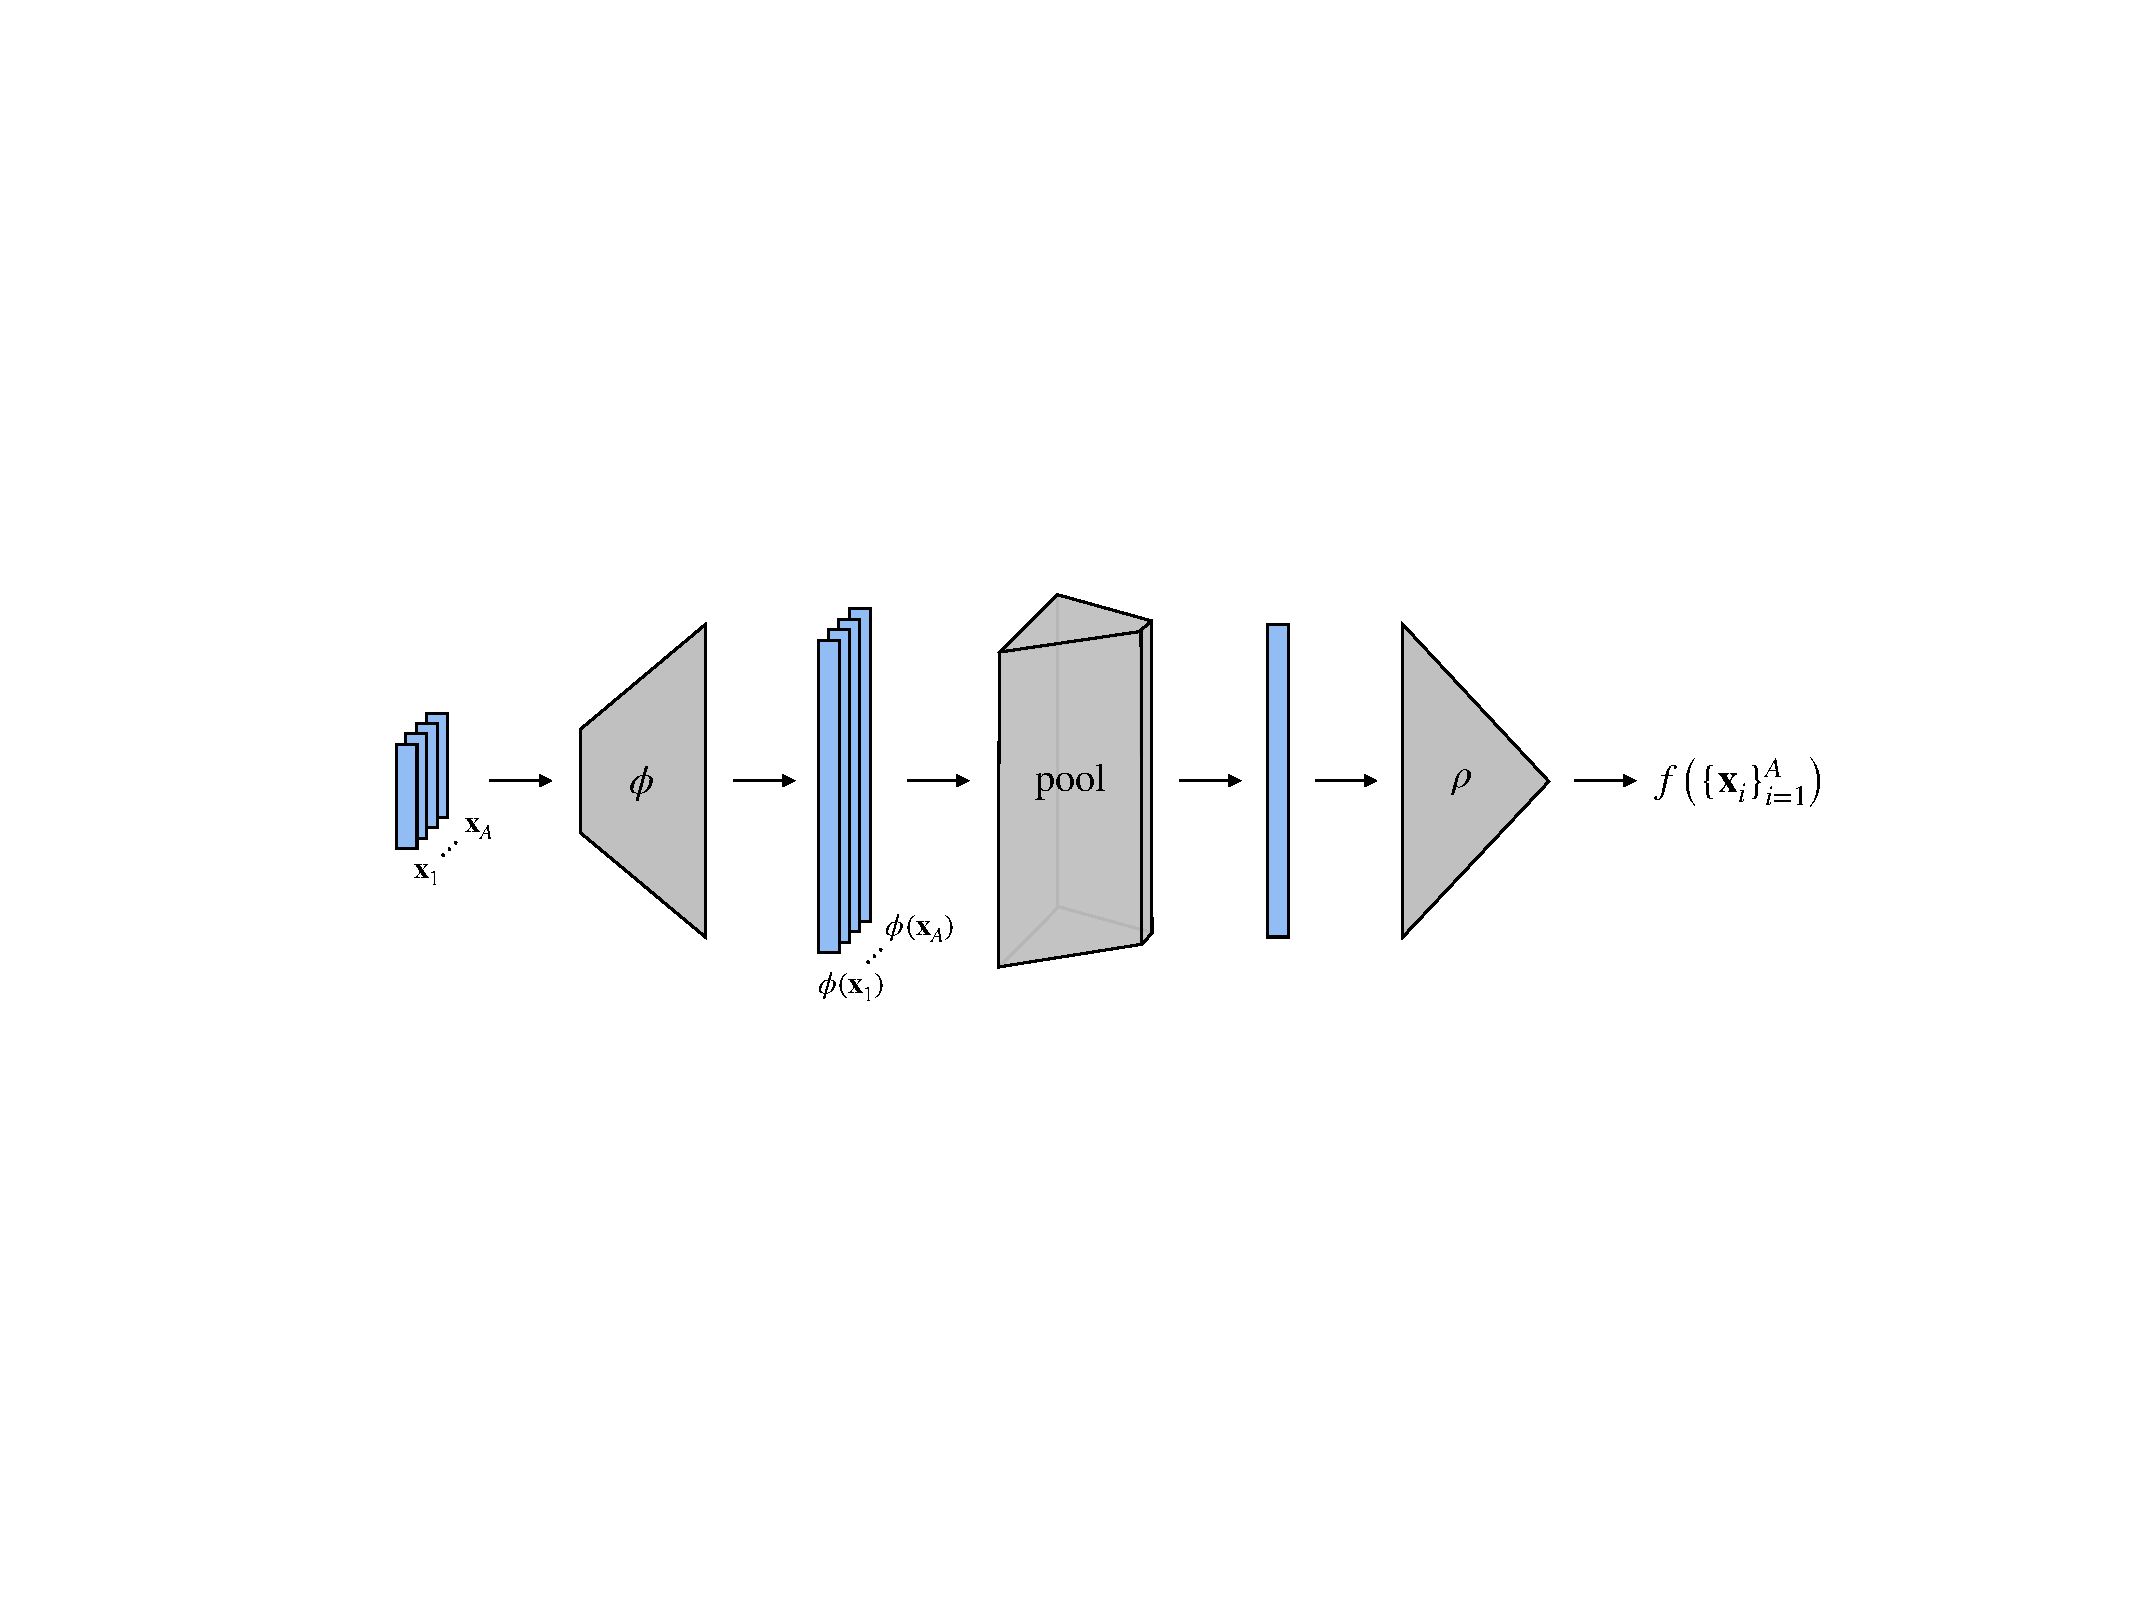
\includegraphics[width=0.75\textwidth,trim=2.5in 4in 2in 3.7in,clip]{figures/neural_quantum_states/deepset.pdf}
    \caption{Cartoon of a Deep Set architecture (adapted from Ref.~\cite{fuchs_deepsets_2019})}
    \label{fig:deepset}
\end{figure}

A wide range of architectural components can be incorporated to further enhance the flexibility and expressive power of neural networks. One prominent example is the use of attention mechanisms~\cite{vaswani_attention_2017}, which dynamically weigh the importance of different elements in an input sequence when making predictions.
Instead of processing all input features equally, attention allows the network to focus selectively on the most relevant parts, effectively learning context-dependent weighting. They form the foundation of modern large language models, enabling them to capture long-range dependencies and nuanced contextual relationships, and have recently been incorporated into neural quantum state architectures to enhance the representation of complex correlations in many-body wavefunctions~\cite{von_glehn_self-attention_2022,pescia_message-passing_2024,geier_self-attention_2025}.


The standard formulation of the self-attention mechanism~\cite{vaswani_attention_2017}
computes queries, keys and values for each element of the input through linear
transformations,
\begin{equation}
    Q = X W_Q, \hspace{1cm} 
    K = X W_K, \hspace{1cm} 
    V = X W_V .
\label{eq:attn-weights}
\end{equation}
As a minimal example, consider the input matrix $X \in \mathbb{R}^{A \times 5}$, chosen to represent the row-wise collection of all single-nucleon degrees of freedom, corresponding to the three spatial coordinates together with the spin and isospin labels. One could alternatively construct $X$ to represent pair degrees of freedom or, more generally, the output of a preceding neural network layer.
Choosing the query and key weight matrices $W_Q$ and $W_K$ to have dimension
$5 \times d_k$, the value weight matrix $W_V$ will have dimension
$5 \times d_v$, yielding $Q, K \in \mathbb{R}^{A \times d_k}$ and
$V \in \mathbb{R}^{A \times d_v}$.
The output of the attention layer is obtained by comparing the query of each particle with the keys of all others, producing a set of normalized weights that are then applied to the values to generate a context-aware representation,
\begin{equation}
    \mathrm{attn}(Q, K, V)
    = \mathrm{softmax}_i \!\left( \frac{Q K^T}{\sqrt{d_k}} \right) V .
\end{equation}
The intermediate matrix $QK^T \in \mathbb{R}^{A \times A}$ encodes all pairwise
similarities between particles and is effectively bilinear in $X$. The row-wise
$\mathrm{softmax}_i$ activation function converts each row into a normalized probability
distribution, and the factor of $1/\sqrt{d_k}$ aids numerical stability.



\subsection{Wave function ansätze}
\label{sec:wavefunction}
Here we review the principal wave function ansätze that have been used in ``first-quantized'' NQS approaches to nuclear physics. These architectures act directly on the continuous spatial coordinates and spin–isospin degrees of freedom of the nucleons.

\subsubsection{Slater--Jastrow}
\label{subsub:slater_jastrow}
Initial applications of the NQS framework to atomic nuclei~\cite{adams_variational_2021}
extended the Slater--Jastrow (SJ) architecture, originally developed for quantum
chemistry~\cite{hermann_deep-neural-network_2020,pfau_ab_2020}, to handle the
complex spin--isospin structure of nuclear interactions. Such an ansatz can be
schematically written as
\begin{equation}
\Psi_{\rm SJ}(X) = F(X)\,\Phi(X)\,,
\label{eq:SJ}
\end{equation}
where $F(X)$ is a permutation-invariant Jastrow factor, and antisymmetry is
enforced by the mean-field-like component $\Phi(X)$. 
For compactness, we use $X=(x_1, \ldots, x_A)$ to denote the collection of all single-particle degrees of freedom $x_i = (\mathbf{r}_i, s_i^z, t_i^z)$, namely the three-dimensional spatial coordinates $\mathbf{r}_i$ and the spin and isospin projections along the $z$-axis.

The mean-field term $\Phi(X)$ is typically expressed as a sum of Slater determinants of single-particle orbitals~\cite{adams_variational_2021,gnech_calculation_2020,yang_consistent_2022}. For atomic nuclei, it takes the form
\begin{equation}
\Phi(X)
= \Bigg[\sum_\mu C_\mu \,
\mathcal{A}\!\left[\phi_{\alpha_1^\mu}(x_1)\,\phi_{\alpha_2^\mu}(x_2)\cdots 
\phi_{\alpha_A^\mu}(x_A)\right]\Bigg]_{J^\pi T}\!,
\label{eq:mf}
\end{equation}
where $\mathcal{A}$ is the antisymmetrization operator acting on the particle labels $x_i$, and $\{C_\mu\}$ are configuration amplitudes that incorporate the Clebsch--Gordan couplings required to form a many-body state $\mu$ with the desired total angular momentum, parity, and isospin $J^\pi T$ for the nucleus of interest. The single-particle orbitals are evaluated as
\begin{equation}
\phi_{\alpha}(x_i) 
= \mathcal{R}_{n l}(r_i)\, Y_{l\,l^z}(\hat{r}_i)\,
\langle s_i^z | s^z \rangle \,
\langle t_i^z | t^z \rangle \, ,
\label{eq:single_particle_nuclei}
\end{equation}
where $\alpha = (n, l, l^z, s^z, t^z)$ are the quantum numbers, 
$\langle s_i^z | s^z \rangle = \delta_{s_i^z,s^z}$ and 
$\langle t_i^z | t^z \rangle = \delta_{t_i^z,t^z}$ project onto the fixed spin and isospin, $\mathcal{R}_{nl}(r_i)$ are the 
radial functions parametrized by MLPs, and $Y_{l\,l^z}(\hat{r}_i)$ are the spherical harmonics. 




\iffalse
% please check the notation of this passage, which I have reworked above
The mean-field part is typically expressed as a sum of Slater determinants of
single-particle orbitals~\cite{adams_variational_2021,gnech_calculation_2020,yang_consistent_2022}. For atomic nuclei, it takes the form
\begin{equation}
\Phi(X)
= \Bigg[\sum_n C_n\,
\mathcal{A}\!\left[\phi_{\alpha_1}(x_1)\,\phi_{\alpha_2}(x_2)\cdots \phi_{\alpha_A}(x_A)\right]\Bigg]_{J^\pi T}\!,
\label{eq:mf}
\end{equation}
where $\mathcal{A}$ is the antisymmetrization operator and $\{C_n\}$ are the
Clebsch--Gordan coupling coefficients chosen so that the state has the desired
total angular momentum, parity, and isospin $(J^\pi, T)$ for the nucleus of interest. The single-particle orbitals are given by
\begin{equation}
\phi_{\alpha_i}(x_i) = \mathcal{R}_{nl}(r_i) Y_{ll_z}(\hat{r}_i) \chi(s^z_i) \eta (t_i^z)\, ,
\label{eq:single_particle_nuclei}
\end{equation}
where $\mathcal{R}_{nl}(r_i)$ are the radial functions parametrized by MLPs, $Y_{ll_z}(\hat{r}_i)$ are the spherical harmonics, and $\chi(s^z_i)$ and $\eta (t_i^z)$ are the spinors describing the spin and isospin of the single-particle state.  To automatically remove the spurious center of mass contribution from the kinetic energy, the spatial coordinates are replaced by $\mathbf{r}_i \to \mathbf{r}_i - \mathbf{R}_{\rm CM}$, with $\mathbf{R}_{\rm CM} = \frac{1}{A}\sum_i \mathbf{r}_i$ being the center of mass coordinate~\cite{massella_exact_2020}. 
\fi

To automatically remove the spurious center-of-mass contribution from the kinetic energy, the spatial coordinates are replaced by $\mathbf{r}_i \to \mathbf{r}_i - \mathbf{R}_{\rm CM}$, with
$\mathbf{R}_{\rm CM} = \frac{1}{A}\sum_{i=1}^A \mathbf{r}_i$
being the center-of-mass coordinate~\cite{massella_exact_2020}.
Since the network parameters are randomly initialized, in the early stages of
training the Metropolis--Hastings walk can let the nucleons drift away from
$\mathbf{R}_{\mathrm{CM}}$. To control this behavior, a Gaussian factor is
multiplied by the single-particle radial functions to confine the nucleons
within a finite volume,
\begin{equation}
\mathcal{R}_{nl}(r_i) \;\to\; \mathcal{R}_{nl}(r_i)\, e^{-\alpha r_i^2}\,.
\end{equation}
Typical values for the confining constant are in the range
$\alpha = 0.02$--$0.05~\text{fm}^{-2}$.

In Refs.~\cite{adams_variational_2021,gnech_calculation_2020,yang_consistent_2022},
the real-valued Jastrow correlator was taken to be of the form
\begin{align}
F(X) = e^{\mathcal{U}(X)}\,\tanh\!\big[\mathcal{V}(X)\big]\,.
\label{eq:jastrow_tanh}
\end{align}
Here, the positive-definite exponential is modulated by a hyperbolic tangent, which acts as a smooth surrogate for the sign. The functions $\mathcal{U}(X)$ and $\mathcal{V}(X)$ are implemented as permutation-invariant neural networks. Several architectures have been developed to represent such functions efficiently, including point-cloud~\cite{charles_pointnet_2017} and attention-based~\cite{vinyals_pointer_2015,vaswani_attention_2017,lee_set_2018}
models. Among these, the authors of Ref.~\cite{adams_variational_2021} found the Deep Sets architecture~\cite{zaheer_deep_2017,wagstaff_limitations_2019} to be a practical and sufficiently accurate choice, discussed further in Section~\ref{sec:deep_learning}.

In particular, each single-particle input $x_i$ is mapped independently to a latent representation, and a sum aggregation is applied to enforce permutation invariance:
\begin{equation}
\mathcal{U}(X)
= \rho_{\mathcal U}\!\left(\sum_{i=1}^A \phi_{\mathcal U}(x_i)\right),
\qquad
\mathcal{V}(X)
= \rho_{\mathcal V}\!\left(\sum_{i=1}^A \phi_{\mathcal V}(x_i)\right).
\label{eq:deep_sets_single}
\end{equation}
Both $\phi_{\mathcal U}$ and $\rho_{\mathcal U}$ (and analogously $\phi_{\mathcal V}$ and $\rho_{\mathcal V}$) are typically implemented as MLPs. Computing the kinetic energy (Laplacian) requires activation functions that are differentiable (ideally twice). Standard choices include hyperbolic tangent, softplus~\cite{dugas_incorporating_2001}, and GELU~\cite{hendrycks_gaussian_2023}.


Instead of single-particle inputs as in Ref.~\cite{adams_sensitivity_2021}, Ref.~\cite{gnech_calculation_2020} maps the coordinates of each particle pair directly to a latent-space representation, in close analogy with earlier condensed-matter applications~\cite{pfau_ab_2020,hermann_deep-neural-network_2020}. As before, a sum aggregation removes any dependence on particle ordering and therefore enforces permutation invariance:
\begin{equation}
\mathcal{U}(X)
= \rho_{\mathcal U}\!\left(\sum_{i \neq j}
\phi_{\mathcal U}(x_i, x_j)\right),
\qquad
\mathcal{V}(X)
= \rho_{\mathcal V}\!\left(\sum_{i \neq j}
\phi_{\mathcal V}(x_i, x_j)\right).
\label{eq:deep_sets_pair}
\end{equation}
When single-particle coordinates are used as input, correlations are generated
in the latent feature space by the aggregation network $\rho_{\mathcal F}$, where we use $\mathcal{F}\in\{\mathcal{U},\mathcal{V}\}$ to
denote either of the two correlator networks. By
contrast, using pair coordinates introduces correlations already at the level of
the real-space inputs. The conventional two-body Jastrow ansatz is recovered
when the latent dimension is one and $\rho_{\mathcal F}$ is taken to be the
identity, $\rho_{\mathcal F}(x)=x$.
In a similar spirit, Ref.~\cite{yang_consistent_2022} feeds only rotationally
invariant one- and two-body features to $\phi_{\mathcal U}$ and
$\phi_{\mathcal V}$, namely $ \|\mathbf r_i \|$, $ \|\mathbf r_j \|$, and
$\| \mathbf r_i-\mathbf r_j \|$, while neglecting spin--isospin dependence. This
choice significantly reduces the number of variational parameters without
compromising the accuracy of the resulting energies.

\subsubsection{Operator-dependent Slater--Jastrow}
\label{sec:chiral_ansatz}

Very recently, VMC methods based on NQS~\cite{yang_chiral_2025,yang_zemach_2025,wen_neural-network_2025} have been applied to the nuclear many-body problem using high-resolution phenomenological and chiral-EFT Hamiltonians that are local in coordinate space. To address the strongly non-perturbative character of these interactions, in particular their tensor component, the NQS includes explicit spin–isospin operator dependence, as in Eq.~\eqref{eq:variational_product}. To keep a polynomial computational cost  in the number of nucleons, the ansatz introduced in Ref.~\cite{yang_chiral_2025} is expressed in the same linearized form used in AFDMC, reported in Eq.~\eqref{eq:variational_linear}, namely
\begin{equation}
\Psi_V(R,S) = e^\mathcal{U}(R) \tanh[\mathcal{V}(R)]
\left( 1 + \sum_{i<j}\sum_{p=1}^6 W^p_{ij}(R) O^p_{ij} \right).
\label{eq:SJ_chiral}
\end{equation}
As a reminder, the first six spin-isospin operators are $O^{p=1,6}_{ij} = \bigl( 1, \tau_{ij}, \sigma_{ij}, \sigma_{ij} \tau_{ij}, S_{ij}, S_{ij} \tau_{ij}\bigr)$. The central correlation functions $\mathcal{U}(R)$ and $\mathcal{V}(R)$ are represented by the spin–isospin independent permutation-invariant neural network of Eq.~\eqref{eq:deep_sets_pair}, introduced in Ref.~\cite{yang_consistent_2022}. Importantly, this construction ensures both translational and rotational invariance. 

Contrary to conventional GFMC and AFDMC trial wave functions, in which the pair
correlation functions $W^p_{ij}$ depend only on the relative coordinate of
particles $i$ and $j$, the present ansatz makes $W^p_{ij}$ a functional of the
full configuration $R$. This is achieved using the Deep Sets architecture, discussed above and in Section~\ref{sec:deep_learning}, which incorporates information from all particles through
\begin{equation}
W^p_{ij}(R) =
\rho_{\mathcal{W}}^p\!\left(
\sum_{k=1}^A \phi_{\mathcal{W}}(r_{ik}, r_{jk}, r_{ij})
\right),
\label{eq:SJ_chiral_2}
\end{equation}
where $\phi_{\mathcal{W}}$ and $\rho_{\mathcal{W}}$ are feedforward neural networks, each with a single fully connected hidden layer. This global dependence allows the pair correlations to adapt to the surrounding many-body environment. As a result, these wave functions provide an excellent starting point for GFMC calculations and were used in Ref.~\cite{yang_chiral_2025} to compute peripheral neutron--$\alpha$ scattering with high accuracy. A more detailed discussion of these results is given in Section~\ref{sec:applications}.



A similar ansatz, but incorporating the \emph{symmetrized product of two-body correlations}---see Eq.~\eqref{eq:variational_product} for its conventional counterpart---has been proposed by the authors of Ref.~\cite{wen_neural-network_2025}:
\begin{equation}
\Psi_V(R,S) =
\left( 1 + \sum_{i<j<k} F_{ijk} \right)
\prod_{i<j} f^c_{ij}(R)
\left( 1 + \sum_{p=2}^6 u_{ij}^p(R)\, O_{ij}^p \right).
\label{eq:wen_ansatz}
\end{equation}
The three-body correlation functions $F_{ijk}$ are defined analogously to
Eq.~\eqref{eq:three_body_corr}. As in the ansatz of Ref.~\cite{wen_neural-network_2025},
\emph{all} radial functions entering the two- and three-body correlations depend on the full
configuration $R$. A representative example is the operator-dependent correlation,
\begin{equation}
u_{ij}^p(R) =
\rho_u^p\!\left(
r_{ij},\,
\sum_{k\neq i,j}
\left[\, \phi_u(r_{ij}) + \phi_u(r_{ik}) \,\right]
\right),
\label{eq:wen_u_corr}
\end{equation}
where both $\rho_u^p$ and $\phi_u$ are feed-forward neural networks composed of multiple one-dimensional transformation layers connected by residual blocks and employing the RiLU activation function.

An important difference from previous NQS implementations is that this approach leverages normalizing flows to produce uncorrelated samples to solve the nuclear Schr\"odinger equation, as opposed to Metropolis–Hastings sampling. As a consequence, it avoids the autocorrelation issues inherent in Metropolis–Hastings and reduces the overall computational cost.
Normalizing flows~\cite{albergo_flow-based_2019,brady_normalizing_2021,wen_application_2024} generate samples by drawing an initial batch from a simple uniform distribution, implemented here using a Sobol quasi-random sequence, and passing it through a series of invertible change-of-variable transformations with tractable derivatives and Jacobians. By optimizing the parameters of the flow, the resulting distribution can be made to closely approximate the target distribution.
Results for the $A=3$ nuclei obtained with this ansatz and the local chiral-EFT interactions of Ref.~\cite{gezerlis_local_2014} will also be summarized in Section~\ref{sec:applications}.

\subsubsection{Hidden Nucleons}
\label{subsub:hidden_nucleons}
A systematically improvable family of variational wave functions for strongly correlated fermionic systems was introduced in Ref.~\cite{moreno_fermionic_2022}. These wave functions are built from Slater determinants in an augmented Hilbert space that includes additional, ``hidden'' fermionic degrees of freedom. The authors demonstrated that this ansatz is universal on the lattice and applied it to the ground-state properties of the Hubbard model on the square lattice, achieving accuracies competitive with state-of-the-art variational methods.
This framework was subsequently extended to nuclear systems, whose Hilbert spaces involve both continuous and discrete degrees of freedom~\cite{lovato_hidden-nucleons_2022}. In this formulation, the Hilbert space includes fictitious coordinates for $A_h$ Hidden Nucleons (HN), defined as functions of the visible coordinates $X_h = f(X)$. The amplitudes of the HN wave function in the $X$ basis can be written schematically as
\begin{equation} 
\Psi_{\rm HN}(X)\equiv \det 
\begin{bmatrix} \Phi_v(X) & \Phi_v(X_h)\\ \chi_h(X) & \chi_h(X_h)\\ \end{bmatrix} ,
\label{eq:HN} 
\end{equation}
where $\Phi_v(X)$ denotes the $A\times A$ matrix of visible single-particle orbitals evaluated at the visible coordinates, equivalent to the mean-field term $\Phi(X)$ of Eq.~\eqref{eq:mf}. This would be the only component of the wave function in a Hartree–Fock description. In contrast to the original implementation of Ref.~\cite{moreno_fermionic_2022}, the columns of the matrix in Eq.~\eqref{eq:HN} correspond to different particles, while the rows correspond to different single-particle states. The $A_h\times A_h$ matrix $\chi_h(X_h)$ contains the amplitudes of hidden orbitals evaluated at hidden coordinates, whereas $\chi_h(X)$ and $\Phi_v(X_h)$ provide the amplitudes of hidden orbitals at visible coordinates and visible orbitals at hidden coordinates, respectively.
The SJ ansatz of Eq.~\eqref{eq:SJ} is recovered in the limit $A_h=1$, $\chi_h(X)=0$, and $\Phi_v(X_h)=0$, allowing one to interpret it as a special case of the HN formulation. If the function $f$ is permutation invariant, $\Psi_{\rm HN}(X)$ is automatically antisymmetric under particle exchange. The expressivity of this construction for discrete degrees of freedom was formally proven in Ref.~\cite{moreno_fermionic_2022}, provided that the functions $\chi_h$ and $f$ are sufficiently general. To avoid the combinatorial complexity of $f$, the $i$-th columns of $\Phi_v(X_h)$ and $\chi_h(X_h)$ are parametrized by independent, permutation-invariant neural networks as
\begin{equation}
\Phi_v^i(X_h) = e^{\mathcal{U}^i_\Phi(X)}\tanh[\mathcal{V}^i_\Phi(X)], \qquad
\chi_h^i(X_h) = e^{\mathcal{U}^i_\chi(X)}\tanh[\mathcal{V}^i_\chi(X)].
\end{equation}
A more recent implementations of the HN ansatz~\cite{gnech_distilling_2024} employs complex-valued matrices of the form
\begin{equation}
\Phi_v^i(X_h) = e^{\mathcal{U}^i_\Phi(X) + i \mathcal{V}^i_\Phi(X)}, \qquad
\chi_h^i(X_h) = e^{\mathcal{U}^i_\chi(X) + i \mathcal{V}^i_\chi(X)}.
\end{equation}
In both formulations, permutation invariance is enforced using Deep Sets architectures~\cite{zaheer_deep_2017,wagstaff_limitations_2019} to express the functions $\mathcal{U}^i_\Phi$, $\mathcal{V}^i_\Phi$, $\mathcal{U}^i_\chi$, and $\mathcal{V}^i_\chi$. For applications to finite nuclei~\cite{lovato_hidden-nucleons_2022} and dilute neutron matter~\cite{fore2023}, a $\mathrm{logsumexp}$ pooling operation replaces the simple sums in Eqs.~\eqref{eq:deep_sets_single} and~\eqref{eq:deep_sets_pair},
\begin{equation}
\mathcal{F}(X)= \rho_\mathcal{F}\left[\log\Big(\sum_i e^{\phi_\mathcal{F}(x_i)}\Big)\right]\,.
\end{equation}
In these works, $\phi_\mathcal{F}$ and $\rho_\mathcal{F}$ are implemented as MLPs with two hidden layers of 16 nodes each, and a 16-dimensional latent space connecting them. The output layers of $\rho_\mathcal{F}$ contain $A$ nodes for $\mathcal{F}=\mathcal{U}^i_\Phi,\mathcal{V}^i_\Phi$ and $A_h$ nodes for $\mathcal{F}=\mathcal{U}^i_\chi,\mathcal{V}^i_\chi$. An ablation study in Ref.~\cite{lovato_hidden-nucleons_2022} examined the convergence of the $^4$He ground-state energy with network size and found that increasing the number of hidden layers or nodes beyond this configuration provided no substantial improvement, while smaller networks slightly degraded the accuracy (by about 0.2 MeV).
The single-particle orbitals defining $\Phi_v(X)$ and $\chi_h(X)$ are also represented by MLPs that take as input the single-particle coordinates $x_i$. In Refs.~\cite{lovato_hidden-nucleons_2022,fore2023}, these networks had two hidden layers with ten nodes each, $\tanh$ activation functions, and one-dimensional linear outputs. Other differentiable activations such as $\mathrm{softplus}$ and $\mathrm{GELU}$ were tested without appreciable differences. Differentiability is required to compute the kinetic energy, which involves second derivatives of the wave function.
Unlike in the Slater–Jastrow case, confinement is not imposed at the single-particle level. Instead, the full wave function in Eq.~\eqref{eq:HN} is multiplied by a global Gaussian factor,
\begin{equation}
\Psi_{\rm HN} (X) \to \Psi_{\rm HN} (X), e^{-\alpha \sum_{i=1}^A r_i^2}\,,
\end{equation}
which ensures spatial localization of the system.

When introducing the HN ansatz, the authors of Ref.~\cite{lovato_hidden-nucleons_2022} found it beneficial
to enforce point symmetries, such as parity and time reversal. For positive- and negative-parity states, one can impose
\begin{align}
\Psi_{\rm HN}^{P^+}(X) &= \Psi_{\rm HN}(R,S) + \Psi_{\rm HN}(-R,S)\,, \nonumber\\
\Psi_{\rm HN}^{P^-}(X) &= \Psi_{\rm HN}(R,S) - \Psi_{\rm HN}(-R,S)\,.
\label{eq:psi_P}
\end{align}
For even-even nuclei, such as $^4$He and $^{16}$O, it is also possible to enforce time-reversal symmetry,
\begin{align}
\Psi_{\rm HN}^{T}(X) \equiv \Psi_{\rm HN}(R,S) + \Psi_{\rm HN}^{*}(R,\theta S)\,.
\label{eq:psi_PT}
\end{align}
where $\theta S$ is obtained by applying the operator $-i\sigma_y$ to all single-particle spinors~\cite{bohr_nuclear_1998}.
Note that, unlike the expression reported in Ref.~\cite{lovato_hidden-nucleons_2022}, we explicitly take the complex conjugate, so that the construction applies to both real- and complex-valued NQS. Importantly, time reversal and parity have been combined, to form a simultaneous eigenstate of parity and time reversal, dubbed $\Psi_{\rm HN}^{PT}(X)$. 

The convergence of the $^4$He ground-state energy computed with $A_h = 4$ HN is displayed in Fig.~\ref{fig:4He}. The parity-conserving wave function $\Psi_{HN}^{P}(R,S)$ is outperformed by $\Psi_{HN}^{PT}(R,S)$, which additionally preserves time-reversal symmetry. Both provide significantly better energies than the SJ results of Ref.~\cite{Gnech2021}, as they can improve the nodal surface of the single-particle Slater determinant. In fact, $\Psi_{\rm HN}^{PT}(R,S)$ yields a variational energy consistent with the numerically exact HH estimate of Ref.~\cite{Gnech2021}. 

It is worth noting that $\Psi_{HN}^{P}(R,S)$ should, in principle, converge to the exact energy, but this may require wider (or deeper) architectures.
To illustrate this point, the right panel of Fig.~\ref{fig:4He} displays the training of $\Psi_{HN}^{P}(R,S)$ with $A_h=4$, in which the number of nodes in the hidden layers of $\phi_\mathcal{F}$ and $\rho_\mathcal{F}$ has been increased from $16$ to $24$. After about $4800$ optimization steps, the parity-conserving ansatz yields energies that are consistent with the HH method. 
Importantly, though,
enforcing time-reversal symmetry in the ansatz is effective in reducing the training time and appears to enhance the expressivity of the HN ANN architecture.

\begin{figure}[!tb]
\begin{center}
    \raisebox{0.4mm}{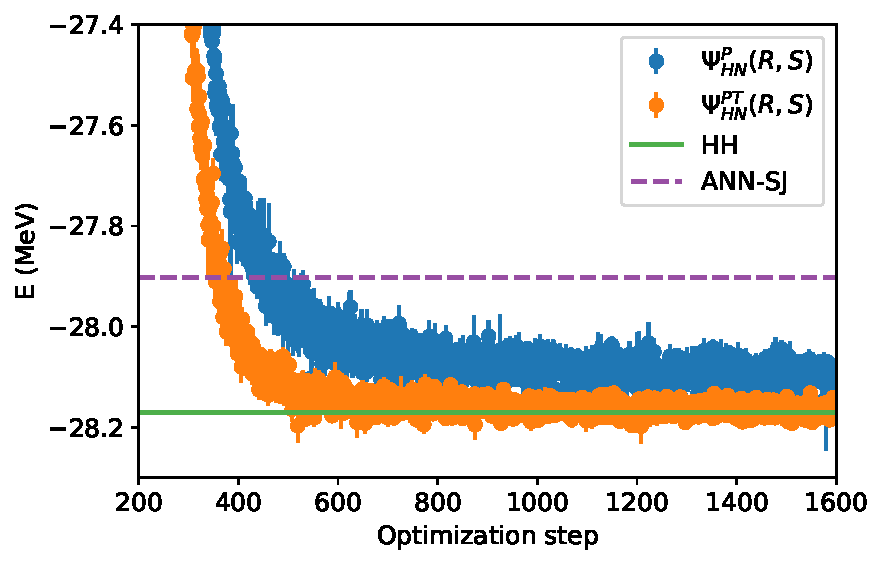
\includegraphics[width=0.49\textwidth, height=0.325\textwidth]{figures/neural_quantum_states/he4_energies.pdf}} 
    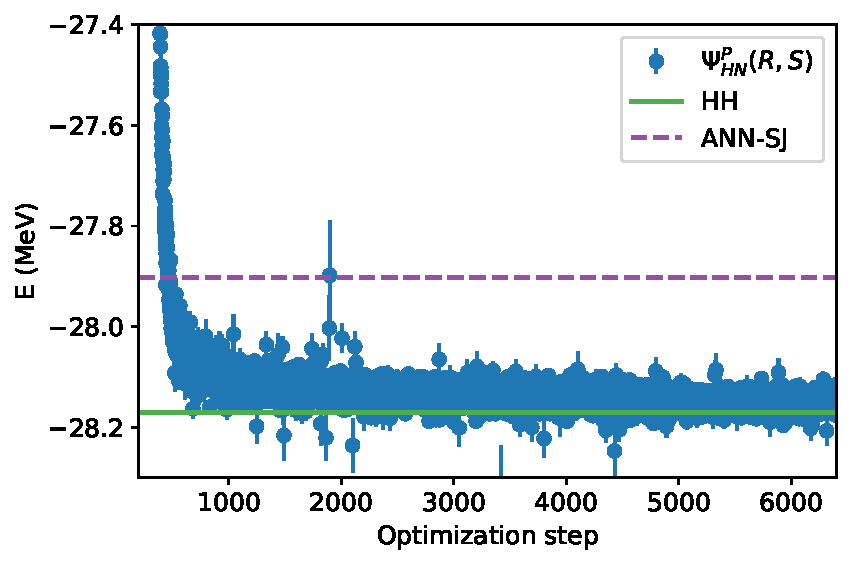
\includegraphics[width=0.49\textwidth]{figures/neural_quantum_states/he4_energies_large.pdf} 
    \caption{From Ref.~\cite{lovato_hidden-nucleons_2022} with permission from the Authors. Left panel: Convergence of the $^4$He ground-state energy obtained with the parity-projected HN ansatz (blue solid circles) and with the ansatz that enforces both parity and time-reversal symmetry (orange solid circles). The SJ and the hyper-spherical harmonics ground-state energies from Ref.~\cite{gnech_calculation_2020} are shown by the purple dashed and solid green lines, respectively.
    Right panel: Convergence of the parity-projected ansatz when employing a wider neural-network architecture than in the left panel.}
    \label{fig:4He}
\end{center}
\end{figure}




\subsubsection{Pfaffian--Jastrow}
\label{subsub:pfaffian_jastrow}


Pfaffian--Jastrow neural architectures were originally introduced to describe the unitary Fermi gas~\cite{kim_neural-network_2024}, where strong pairing correlations dominate. The same pairing-based formulation was later shown to be advantageous for nuclei and dilute neutron-star matter~\cite{fore_investigating_2024}. These neural architectures build on a long history of pairing wave functions in quantum Monte Carlo studies of ultracold Fermi gases, in which the many-body state is written as an antisymmetrized product of spin-singlet pairs~\cite{gezerlis_strongly_2008,carlson_superfluid_2003,chang_quantum_2004,gezerlis_heavy-light_2009}. These can be thought of as Bardeen--Cooper--Schrieffer (BCS) pairs within the nuclear context.

In the literature, this class of pairing states appears under several closely related names, including geminal wave functions~\cite{casula_geminal_2003,casula_correlated_2004}, number-projected BCS~\cite{galea_diffusion_2016}, and singlet-pairing wave functions~\cite{bajdich_pfaffian_2008}. These ansätze already provide a substantial improvement over single-determinant Slater states. However, their effectiveness is reduced in partially spin-polarized systems, since only the spin-singlet pairing channel is included~\cite{casula_correlated_2004}. This limitation motivated the introduction of the singlet–triplet–unpaired (STU) Pfaffian wave function~\cite{bajdich_pfaffian_2006,bajdich_pfaffian_2008}, which generalizes the geminal form by explicitly incorporating both singlet and triplet pairing channels, together with a separate sector for unpaired particles. In this formulation, the many-body wave function is written as the Pfaffian of a block matrix collecting singlet, triplet, and unpaired contributions. The original geminal ansatz is recovered as a special case when the triplet blocks are set to zero.

A key limitation of both geminal and STU wave functions in their original formulations is that they assume a fixed spin ordering of the fermions. This is perfectly adequate for model Hamiltonians with conserved spin species, but it is not well suited to nuclear interactions, which contain explicit spin-exchange terms and couple different spin–isospin channels~\cite{piarulli_local_2020}. In neutron-matter applications, this issue is commonly circumvented by expressing the Pfaffian pairing orbital as a plane-wave expansion weighted by BCS amplitudes and multiplied by a spin-singlet component~\cite{Gandolfi2009}:
\begin{equation}
\phi(x_i, x_j)
= \sum_{\alpha} c_{\alpha} \,
e^{i \mathbf{k}_{\alpha} \cdot (\mathbf{r}_i - \mathbf{r}_j)}\,\left(
\frac{\eta_\uparrow(s_i^z)\eta_\downarrow(s_j^z)
      - \eta_\downarrow(s_i^z)\eta_\uparrow(s_j^z)}{\sqrt{2}}\right) \, ,
\label{eq:pf_pairing_orbital_nm}
\end{equation}
where $x_i = (\mathbf{r}_i, s_i^z)$,
$\mathbf{k}_{\alpha} = \tfrac{2\pi}{L}(n_x \hat{\mathbf{x}} + n_y \hat{\mathbf{y}} + n_z \hat{\mathbf{z}})$
denotes the momenta compatible with the periodic boundary conditions, and the complex-valued $c_{\alpha}$ are variational parameters. While in neutron matter the spin-triplet channel is typically neglected, it can be incorporated within the same framework without requiring fixed spin ordering.

By introducing neural network representations of the pairing orbital, the Pfaffian can be employed in its most general form, capturing arbitrary spin–isospin–dependent correlations without relying on fixed assumptions about the pairing channel.
For an even number of nucleons $A$, the Pfaffian--Jastrow wave function is written as
\begin{equation}
\Psi_{PJ}^{\mathrm{even}}(X) = e^{J(X)}\, \mathrm{pf}[P(X)]\,,
\label{eq:pf_even}
\end{equation}
where $J(X)$ is a Jastrow factor and $P(X)$ is an $A \times A$ skew-symmetric matrix whose elements define the pairing orbital between any two nucleons.
The antisymmetric structure of the wave function is thus fully encoded in the pairing matrix $P(X)$, given by~\cite{kim_neural-network_2024,fore_investigating_2024}
\begin{equation}
P(X) =
\begin{bmatrix}
0 & \phi(x_1,x_2) & \phi(x_1,x_3) & \cdots & \phi(x_1,x_A) \\
-\phi(x_1,x_2) & 0 & \phi(x_2,x_3) & \cdots & \phi(x_2,x_A) \\
-\phi(x_1,x_3) & -\phi(x_2,x_3) & 0 & \cdots & \phi(x_3,x_A) \\
\vdots & \vdots & \vdots & \ddots & \vdots \\
-\phi(x_1,x_A) & -\phi(x_2,x_A) & -\phi(x_3,x_A) & \cdots & 0
\end{bmatrix} \, .
\end{equation}
Similarly to the most recent implementations of the HN ansatz, the Jastrow factor is complex-valued~\cite{fore_investigating_2024} and can be written as
\begin{align}
F(X) = e^{\left[\mathcal{U}(X) + i\mathcal{V}(X)\right]}\,,
\label{eq:jastrow_complex}
\end{align}
where $\mathcal{U}$ and $\mathcal{V}$ are real functions that encode two-body correlations in the modulus and phase of the wave function, respectively.
As in the real-valued case, the pairwise Deep-Sets construction of Eq.~\eqref{eq:deep_sets_pair} is typically employed, so that two-body correlations are built directly in coordinate space rather than in the latent feature space.


Alternatively, the pairing orbital can be taken to be a sum over products of single-particle orbitals,
\begin{equation}
\phi(x_i, x_j)
= \sum_{\alpha, \beta} c_{\alpha\beta} \, \phi_{\alpha}^*(x_i)\, \phi_{\beta}(x_j)\,,
\label{eq:pf_pairing_orbital_closed}
\end{equation}
where the single-particle orbitals $\phi_{\alpha}(x)$ are those defined in Eq.~\eqref{eq:single_particle_nuclei}. This strategy has also been adopted in recent condensed-matter applications of the Pfaffian family of wave functions~\cite{gao_neural_2024}, where the elements of the antisymmetric matrix $c_{\alpha\beta}$ are treated as variational parameters. For a closed-shell system, the Slater–Jastrow ansatz is recovered by restricting the sum to the occupied orbitals and choosing $c_{\alpha\beta}$ to be antisymmetric and nonzero only between time-reversed partners $(\alpha, \bar{\alpha})$, e.g. $c_{\alpha \bar{\alpha}} = 1$,  $c_{\bar{\alpha} \alpha} = -1$, with all other $c_{\alpha\beta}=0$. This choice forms antisymmetric pairs of conjugate single-particle states (the usual time-reversed pairs of a closed shell), and in this limit the Pfaffian reduces to the determinant built from the same one-body orbitals, thus recovering the SJ form as a special case.

In contrast to these orbital-product expansions, and to both the SJ and HN ansätze, one can require only a single trainable pair orbital $\phi$, so the number of variational parameters does not grow with the number of particles $A$. Skew-symmetry is enforced at the level of the orbital itself by parameterizing $\phi$ through a neural network $\nu$,
\begin{equation}
\phi(x_i, x_j)
= \nu(x_i, x_j) - \nu(x_j, x_i)\,,
\end{equation}
so that $\phi(x_i, x_j) = - \phi(x_j, x_i)$ holds identically. In practice~\cite{kim_neural-network_2024,fore_investigating_2024}, $\nu$ is implemented as an MLP acting on the concatenated features of the two nucleons, which allows the orbital to depend simultaneously on relative position and on spin–isospin quantum numbers, thereby capturing correlations beyond pure pairing.

For systems with an odd number of nucleons, the ansatz is extended by adding a single unpaired orbital $\psi$, parameterized by a separate MLP. In this case, the Pfaffian is taken over an enlarged $(A+1)\times(A+1)$ skew-symmetric matrix:
\begin{equation}
\Psi_{PJ}^{\mathrm{odd}}(X)
= e^{J(X)}
\, \mathrm{pf}
\begin{bmatrix}
P(X) & \mathbf{u}(X) \\
-\mathbf{u}(X)^{T} & 0
\end{bmatrix},
\label{eq:pf_odd}
\end{equation}
where
\begin{equation}
\mathbf{u}(X) =
\begin{bmatrix}
\psi(x_1) \ \psi(x_2) \ \cdots \ \psi(x_A)
\end{bmatrix}^T
\end{equation}
collects the values of the unpaired orbital on all single-particle degrees of freedom. This construction preserves antisymmetry while allowing Pfaffian-based NQS to describe odd-mass nuclei or systems with a blocked quasiparticle.

Although the Pfaffian ansatz for odd $A$ introduces an additional, unpaired orbital relative to the even-$A$ case, the overall number of trainable parameters in both formulations remains independent of the particle number. Moreover, because the even- and odd-$A$ constructions share the same underlying pairing orbital, transfer-learning strategies can be straightforwardly employed between neighboring systems. This favorable scaling has enabled simulations of dilute, isospin-asymmetric neutron-star matter with up to $A=42$ nucleons under periodic boundary conditions~\cite{fore_investigating_2024}. Owing to this efficiency, the Pfaffian ansatz is emerging as a particularly effective tool for larger systems, while benchmark studies continue to compare its performance with the HN ansatz, which is known to provide a universal approximation to antisymmetric wave functions~\cite{moreno_fermionic_2022}.

In neutron matter, pairing is an essential ingredient, whereas in finite nuclei it may or may not be dominant, depending on shell structure and interaction strength~\cite{dean_pairing_2003}. Nevertheless, the Pfaffian formulation remains attractive because (i) for an appropriate choice of pairing orbital it collapses to a single Slater determinant; (ii) the orbital depends simultaneously on spatial and spin–isospin coordinates, allowing it to capture independent-pair correlations beyond pure pairing; (iii) it yields a compact description of open-shell systems without resorting to linear combinations of many Slater determinants; and (iv) its cost scales favorably with system size, since only a single pairing orbital is required regardless of $A$.


\subsubsection{Backflow correlations}
\label{subsub:backflow_correlations}

Backflow correlations encode how the state of a single particle is influenced by the coordinates of all the others, effectively redefining its coordinates according to the many-body configuration,
$x_i \mapsto g_i(x_i; \{ x_j\}_{j \neq i})$.
This idea dates back to Ref.~\cite{feynman_energy_1956} and has since become a widely adopted strategy for enhancing the expressivity of antisymmetric NQS~\cite{luo_backflow_2019,hermann_deep-neural-network_2020,pfau_ab_2020}.
A key requirement is permutation equivariance: permuting the particles in the input must produce the same permutation in the output, $g_i \mapsto g_j$ if $x_i \mapsto x_j$, so as to preserve the antisymmetry of the fermionic wave function.

A relatively simple backflow transformation has been recently incorporated into the HN framework and applied to compute properties of nuclei such as $^{20}$Ne in Ref.~\cite{gnech_distilling_2024}.
The equivariant backflow transformation reads
\begin{equation}\label{eq:mpnn}
g_i = \Big(x_i, \sum_j m(x_i, x_j) \Big)\, ,
\end{equation}
with $m$ an MLP made of two fully-connected layers with $32$ nodes each~\cite{gnech_distilling_2024}.

The calculations in Ref.~\cite{Yang:2023rlw} for $^4$He, $^6$Li, and $^{16}$O employ a \emph{multi-determinant} SJ architecture with neural backflow, dubbed \emph{FeynmanNet}.
The backflow transformation generalizes the Fermionic Neural Network of Ref.~\cite{pfau_ab_2020} to encompass both continuous spatial and discrete spin--isospin degrees of freedom.
As shown in Sec.~\ref{sec:applications}, this architecture yields highly accurate ground-state energies for input Hamiltonians from pionless EFT at leading and next-to-leading order, which include a short-range tensor component.

Many nuclear-physics calculations based on NQS make use of transformations built from message-passing neural networks (MPNNs) to improve the flexibility and scalability of the variational ansatz.
MPNN-based backflow was first integrated into the SJ ansatz to preprocess the input coordinates.
In its first application to the homogeneous electron gas, this strategy enabled simulations with up to $N=128$ electrons at extremely low densities~\cite{pescia_message-passing_2024}.
It was later extended to ultracold Fermi gases~\cite{kim_neural-network_2024}, where strong pairing correlations are particularly challenging.
Most recently, MPNNs have been used to compute properties of dilute neutron-star matter, substantially enhancing the expressivity of the PJ ansatz and allowing a first-principles description of cluster formation in the neutron-star crust~\cite{fore_investigating_2024}.

MPNNs are a class of graph neural networks designed to model correlations in graph-structured data. In quantum systems of identical particles, this graph is fully connected, with each particle interacting with every other.
Importantly, to satisfy the Pauli principle, MPNNs can process inputs in a permutation-equivariant manner.
There are many possible ways to implement an MPNN, but the core idea is to iteratively update the information encoded on the nodes and edges of a graph.
The input graph typically encodes single-particle features on the nodes and pairwise features on the edges.
At each iteration, messages are passed along the edges based on these features, allowing each node to incorporate information from its neighbors.
As a result, the node and edge representations become increasingly enriched with nonlocal, correlated information from the entire system.
The output is then another graph with the same connectivity but with node and edge features that encode many-body correlations in a permutation-equivariant way.
These features can then be fed into other parts of the NQS in place of the original node and edge features.


Here, we outline the structure of the MPNN following Ref.~\cite{fore_investigating_2024} based on earlier developments in Refs.~\cite{pescia_message-passing_2024,kim_neural-network_2024}, with modifications appropriate for finite nuclei.
We take the input single-particle ``visible'' features as \( \mathbf{v}_i = [\bar{\mathbf{r}}_i, s_i^z, t_i^z ] \). Note that—unlike in periodic systems, where only the spin and isospin of particle \( i \) are used as inputs—here the Cartesian coordinates of the nucleons are also included. To automatically remove spurious center-of-mass contributions from all observables~\cite{massella_exact_2020}, we define the intrinsic spatial coordinates as \( \bar{\mathbf{r}}_i = \mathbf{r}_i - \mathbf{R}_{\rm CM} \), where \( \mathbf{R}_{\rm CM} \) denotes the center of mass of the nucleus. The ``visible'' pairwise features encode spatial as well as spin–isospin coordinates and are defined by  
\[
\mathbf{v}_{ij} = [ \,\mathbf{r}_i-\mathbf{r}_j, \| \mathbf{r}_i - \mathbf{r}_j \|, s_i^z, s_j^z, t_i^z, t_j^z] \, .
\]

The initial hidden features for the nodes and the edges are obtained by concatenating the original and transformed single-particle and two-particle features, respectively, as
\begin{equation*}
\mathbf{h}_i^{(0)} = [\mathbf{v}_i, f_A(\mathbf{v}_i)] \quad , \quad
\mathbf{h}_{ij}^{(0)} = [\mathbf{v}_{ij}, f_B(\mathbf{v}_{ij})] \, .
\end{equation*}
Here, \( f_A \) and \( f_B \) are MLPs that preprocess the input coordinates and map them into a common latent space, ensuring that the dimensions of the hidden features \( \mathbf{h}_i^{(t)} \) and \( \mathbf{h}_{ij}^{(t)} \) remain independent of the iteration index \( t \).

The MPNN update is performed iteratively for \( t = 1, \dots, T \). At each step, information between the node and edge features is exchanged through the message
\begin{equation}
\mathbf{m}_{ij}^{(t)} = f_M^{(t)}\!\left( \mathbf{h}_i^{(t-1)}, \mathbf{h}_{ij}^{(t-1)}, \mathbf{h}_j^{(t-1)} \right) ,
\label{eq:mpnn-message}
\end{equation}
where \( f_M^{(t)} \) is an MLP. For each particle \( i \), the relevant messages are collected and pooled to eliminate any ordering with respect to the other particles \( j \neq i \). As in Ref.~\cite{kim_neural-network_2024}, we use logsumexp pooling, a smooth alternative to max pooling,
\begin{align*}
\mathbf{m}_{i}^{(t)} = \log\!\left(\sum_{j \neq i} \exp\!\left(\mathbf{m}_{ij}^{(t)}\right)\right) .
\end{align*}
The hidden node and edge features are then updated as
\begin{align*}
\mathbf{h}_i^{(t)} &= \left[ \mathbf{v}_i, f_F^{(t)}\!\left(\mathbf{h}_i^{(t-1)}, \mathbf{m}_{i}^{(t)}\right) \right] , \\
\mathbf{h}_{ij}^{(t)} &= \left[ \mathbf{v}_{ij}, f_G^{(t)}\!\left(\mathbf{h}_{ij}^{(t-1)}, \mathbf{m}_{ij}^{(t)}\right) \right] .
\end{align*}
The functions \( f_M^{(t)} \), \( f_F^{(t)} \), and \( f_G^{(t)} \) are distinct MLPs whose output dimensions match those of \( f_A \) and \( f_B \). Including concatenated skip connections to the visible features ensures that the signal from the raw input remains accessible even as the MPNN depth \( T \) increases.


Finally, after the \( T \)-th iteration, we aggregate the hidden node and edge features into single-particle and pairwise feature vectors:
\begin{align*}
\mathbf{g}_{ij} &= \left[ \mathbf{h}_i^{(T)}, \mathbf{h}_j^{(T)}, \mathbf{h}_{ij}^{(T)} \right] \,, \\ 
\mathbf{g}_i &=  \log\left(\sum_{j \neq i} \exp\left(\mathbf{g}_{ij}\right) \right)\,.
\end{align*}
By construction, \( \mathbf{g}_i \) and \( \mathbf{g}_{ij} \) define a permutation-equivariant
many-body feature embedding of the original single-particle and pairwise degrees of freedom. Rather than representing a fixed coordinate transformation, the MPNN learns a nonlinear, nonlocal reparameterization of the input graph that can be used as a drop-in replacement for the original node and edge features in a wide class of NQS.

In recent works~\cite{kim_neural-network_2024,fore_investigating_2024}, the pairwise features \( \mathbf{g}_{ij} \) are used to parameterize
the Pfaffian pairing orbital and the Jastrow factor, replacing the bare inputs
\( (x_i, x_j) \) with their correlated counterparts. However, this choice is not intrinsic
to the construction: the same embedding can be coupled to SJ~\cite{pescia_message-passing_2024}, HN~\cite{gnech_distilling_2024},
or other operator-based ansätze, and the single-particle features \( \mathbf{g}_i \) may
equally be used to define backflow-modified one-body orbitals. In this sense, the
MPNN provides a general, architecture-agnostic mechanism for incorporating
many-body correlations into neural wave functions.


\begin{figure}[!tb]
\centering
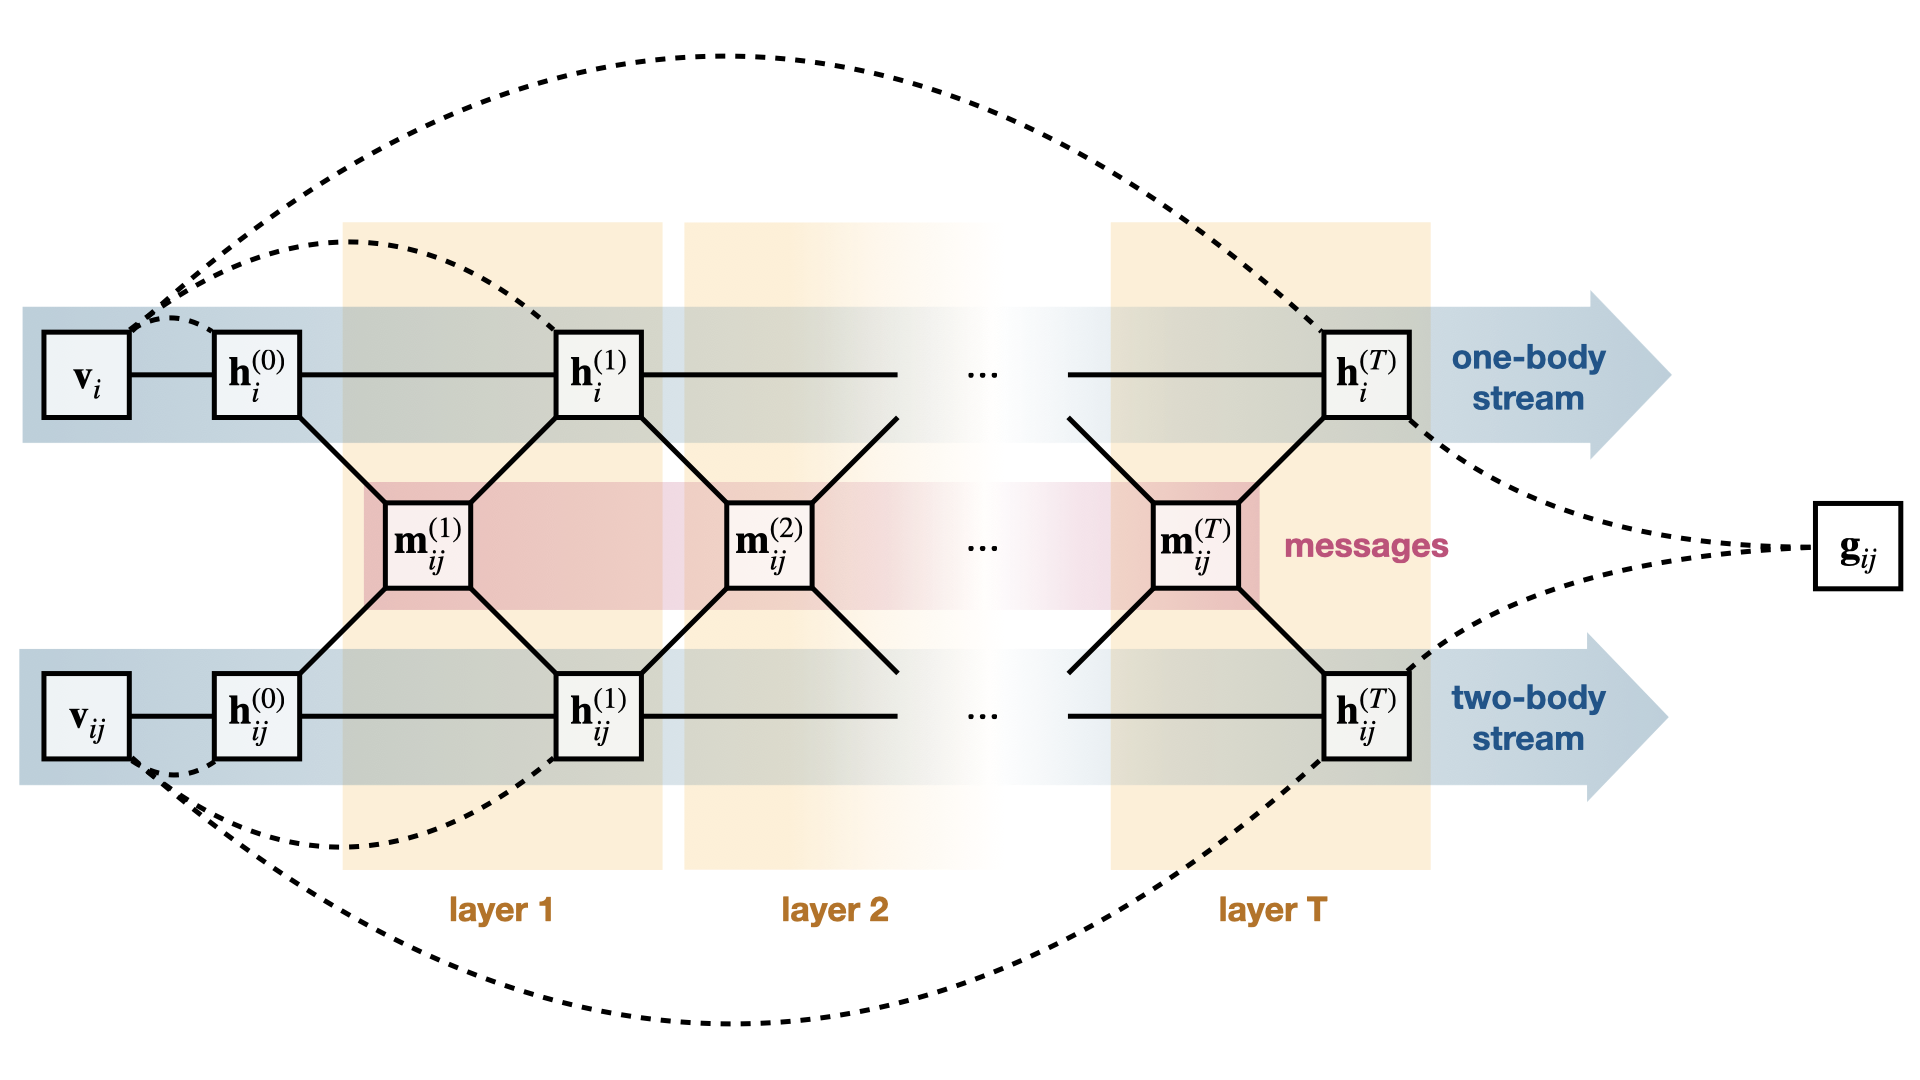
\includegraphics[width=0.95\columnwidth]{figures/overview/MPNN.png}
\caption{Schematic representation of the message-passing neural network. Each of the $T$ total iterations of the network is represented by a yellow box. 
  Dashed lines represent the concatenation operations, while solid lines represent the parameterized transformations (linear transformations and nonlinear feedforward neural networks). Messages, highlighted in pink, mediate the exchange of information between the one- and two-body streams, in blue.}
\label{fig:mpnn}
\end{figure}